\documentclass[11pt,a4paper]{article}
\usepackage[spanish,es-nodecimaldot,es-tabla]{babel}
\usepackage{lmodern}
\usepackage[margin=2.5cm]{geometry}
\usepackage{booktabs,tabularx,multirow,array}
\usepackage{graphicx}
\usepackage{amsmath,amssymb}
\usepackage{xcolor}
\usepackage{tikz}
\usetikzlibrary{arrows.meta,positioning,fit,calc}
\usepackage[labelfont=bf,font=small]{caption}
\usepackage{enumitem}
\usepackage{microtype}
\usepackage[hidelinks]{hyperref}
\usepackage{url}

\setlength{\parindent}{1.5em}
\renewcommand{\arraystretch}{1.12}
\newcolumntype{L}{>{\raggedright\arraybackslash}X}
\graphicspath{{figuras/}}

\title{\textbf{song2game}}
\author{%
\begin{tabular}{c@{\hspace{2.2em}}c}
David Joacim Cervantes Gómez & Alan García Jiménez \\
\texttt{\small davidjoacim1@gmail.com} & \texttt{\small alangj14@gmail.com} \\[6pt]
Enrique García Páez & Gonzalo Sandoval Vásquez \\
\texttt{\small garcia.paez.enrique@gmail.com} & \texttt{\small sandoval.vasquez.gon@gmail.com}
\end{tabular}}
\date{}

\begin{document}
\maketitle

\begin{abstract}
\noindent
Aprender una canción de oído exige separar mentalmente lo que toca cada instrumento y
traducirlo a algo que se pueda leer. song2game automatiza ese proceso: recibe un enlace de
YouTube, descarga el audio, lo separa en seis pistas (voz, batería, bajo, guitarra, piano y otros)
con BS-RoFormer SW, transcribe la mezcla a MIDI con MuScriptor large ---un \emph{Transformer}
de 1{,}4 mil millones de parámetros--- y convierte ese MIDI en tablatura de guitarra, piano
repartido por manos y carriles de batería, que se practican como un juego encima de las pistas
reales. El diseño original preveía un modelo especializado por instrumento; para la batería, el
\emph{nivel~1} era la red convolucional-recurrente de ADTOF, de menos de medio millón de parámetros.
Este reporte documenta ese nivel~1 tal como se evaluó en el cuaderno del proyecto y lo compara con
el modelo que el sistema usa, con la misma métrica, sobre las 23 canciones de MDB-Drums y en tres
condiciones de entrada. La evaluación reproduce exactamente las cifras del cuaderno ($F_1=0{,}742$
en sus 7 canciones de prueba) y muestra que, sobre la pista de batería separada por BS-RoFormer,
ADTOF obtiene el mejor resultado ($F_1=0{,}851$), por encima de MuScriptor sobre la mezcla
($0{,}739$), con unas 28 veces menos tiempo de cómputo. MuScriptor se conserva porque un solo modelo
transcribe los cuatro instrumentos, pero los datos indican que la batería debería volver al diseño
original. El post-proceso de guitarra y piano ---eliminación de \emph{bleed}, clasificación
acorde/notas y digitación por Viterbi, reparto entre dos manos--- está cubierto por 28 pruebas
automáticas que pasan.

\medskip
\noindent\textbf{Palabras clave:} transcripción automática de música, separación de fuentes,
transcripción de batería, ADTOF, MuScriptor, BS-RoFormer, tablatura, MIDI.
\end{abstract}

\noindent\textbf{Idea central: el objetivo es el MIDI, no el audio ni el modelo.} Cada decisión del
proyecto ---qué separador, qué transcriptor, qué limpieza--- se juzga por la calidad de las notas que
llegan a la persona que practica, medida con $F_1$ de notas o golpes, y no por el tamaño del modelo ni
por métricas intermedias como la calidad del audio separado.

% ======================================================================
\section{Introducción}

Quien aprende un instrumento por su cuenta suele hacerlo con canciones que ya conoce. El camino
habitual ---buscar una tablatura en internet o sacar la canción de oído--- tiene dos problemas: las
tablaturas disponibles son de calidad muy variable y no existen para la mayoría de las canciones, y
sacar una parte de oído es difícil cuando el instrumento queda tapado por la voz, el bajo o la
batería. Esta sección plantea el problema, el objetivo y el alcance del trabajo.

\subsection{Planteamiento del problema}

Pasar de una grabación comercial a algo que se pueda practicar combina dos problemas abiertos. El
primero es la \textbf{separación de fuentes musicales}: obtener, a partir de la mezcla, la señal de
cada instrumento. El segundo es la \textbf{transcripción automática de música}: convertir el audio en
notas con inicio, fin, altura y, si es posible, intensidad. Ninguno está resuelto: los mejores
separadores abiertos dejan la guitarra y el piano mucho menos limpios que el bajo y la batería, y los
transcriptores que reconocen varios instrumentos todavía confunden timbres parecidos, como guitarra y
piano. Encima de ambos hay un tercer problema, propio del uso: un archivo MIDI no es una tablatura.
Para guitarra hay que decidir cuerda y traste de cada nota; para piano, qué mano toca cada nota; y
para batería, qué pieza del kit suena en cada golpe.

\subsection{Objetivo y alcance}

El objetivo es construir un sistema de punta a punta que, a partir de un enlace de YouTube, entregue
las pistas separadas y una transcripción practicable de guitarra, piano y batería, sincronizada con el
audio original y presentada como un juego de ritmo. Queda fuera del alcance generar partituras en
notación tradicional, transcribir la voz, funcionar en tiempo real y entrenar modelos grandes desde
cero.

Las contribuciones del trabajo son: (1) un flujo completo ---descarga, separación, transcripción y
post-proceso--- que corre en un contenedor Docker sin GPU; (2) un esquema de \emph{tres pasadas} de
MuScriptor condicionadas por instrumento, con eliminación de notas que otra pista explica mejor;
(3) un post-proceso de guitarra y piano basado en reglas físicas y programación dinámica; (4) la
evaluación del modelo de batería de nivel~1 (ADTOF) sobre tres conjuntos de datos, y (5) una
comparación controlada entre ese modelo y MuScriptor, que revisa la decisión de arquitectura.

% ======================================================================
\section{Trabajos relacionados}

El proyecto se apoya en cuatro líneas de investigación: la separación de fuentes, la transcripción de
instrumentos con altura, la transcripción de batería y la conversión de notas a tablatura. Esta sección
resume el estado del arte de cada una y ubica en ella los modelos elegidos.

\subsection{Separación de fuentes musicales}
La separación moderna parte del \emph{benchmark} MUSDB18, con cuatro pistas: voz, bajo, batería y
otros. Entre 2019 y 2023 la calidad promedio en MUSDB18-HQ pasó de unos 5{,}3~dB de SDR (la métrica se
explica en la sección~\ref{sec:sdr}) con Open-Unmix a 9{,}8~dB con BS-RoFormer entrenado con datos
estándar, y a unos 12~dB con 500 canciones extra, lo que le dio el primer lugar en el Sound Demixing
Challenge 2023~\cite{lu2023bsroformer}. Mel-RoFormer~\cite{wang2023melroformer} cambia la división en
bandas por bandas Mel traslapadas, con mejoras en voz pero resultados inconsistentes en batería y
peores en bajo.

\subsection{Transcripción automática de música}
Tras los métodos de factorización de matrices, la transcripción pasó a redes
convolucionales-recurrentes. Onsets and Frames~\cite{hawthorne2018onsets} separó la detección de
inicios y de notas activas. Después llegaron los \emph{Transformers}: hFT-Transformer alcanzó 97{,}4~\% de
$F_1$ de nota en piano~\cite{toyama2023hft}, y los modelos secuencia-a-secuencia trataron la
transcripción como una traducción de audio a símbolos tipo MIDI~\cite{hawthorne2021seq2seq}.
MT3~\cite{gardner2022mt3} extendió esa idea a varios instrumentos con un vocabulario común, y
MuScriptor~\cite{rouard2026muscriptor} la llevó a gran escala con entrenamiento en datos reales.

\subsection{Transcripción de batería}
La transcripción de batería detecta golpes y su pieza, sin altura ni duración. Vogl et
al.~\cite{vogl2017} propusieron redes convolucionales-recurrentes sobre espectrogramas logarítmicos;
Zehren et al.\ reprodujeron esa arquitectura en ADTOF~\cite{zehren2023adtof} y la entrenaron con 359~h
de música real. E-GMD~\cite{callender2020egmd} aportó 444~h de batería electrónica con intensidad de
cada golpe, y Noise-to-Notes~\cite{yeung2025n2n} planteó la tarea como generación por difusión, con el
mejor resultado publicado. La comparación de Noise-to-Notes (tabla~\ref{tab:publicados}) muestra un
problema de dominio: ADTOF, entrenado con música real, cae a 44{,}95 de $F_1$ en E-GMD, y los modelos
entrenados solo con E-GMD caen a 70--75 en MDB.

\begin{table}[ht]
\centering
\caption{$F_1$ de \emph{onset} publicado (tabla de Noise-to-Notes~\cite{yeung2025n2n}). Cada modelo cae
fuera del dominio con que se entrenó.}
\label{tab:publicados}
\begin{tabular}{llccc}
\toprule
\textbf{Modelo} & \textbf{Entrenado con} & \textbf{E-GMD} & \textbf{MDB} & \textbf{IDMT} \\
\midrule
Onsets and Frames Drums & E-GMD & 83{,}40 & 75{,}19 & 85{,}72 \\
ADTOF & Música real & 44{,}95 & 86{,}87 & 94{,}67 \\
hFT-Transformer adaptado & E-GMD & 86{,}31 & 70{,}81 & 70{,}61 \\
Noise-to-Notes (10 pasos) & E-GMD & 89{,}68 & 87{,}86 & 94{,}90 \\
\bottomrule
\end{tabular}
\end{table}

\subsection{De MIDI a tablatura}
Asignar cuerda y traste es un problema de búsqueda: cada altura tiene varias posiciones posibles y la
mejor depende de las notas vecinas. AutoTab~\cite{matos2025autotab} lo resuelve con caminos más cortos
en grafos, y TART~\cite{gupta2026tart} con un modelo T5 condicionado por audio, con 71{,}8~\% de $F_1$
de tablatura cuando las notas son perfectas y 54{,}1~\% de punta a punta: los errores del paso de audio
a notas se propagan. Este proyecto usa programación dinámica con costos físicos explícitos, más simple
y sin entrenamiento.

% ======================================================================
\section{Marco teórico}

Esta sección reúne los conceptos que se usan en el resto del reporte: cómo se mide la calidad de una
separación y qué significan los decibeles, qué es una pista separada y por qué se contamina con otros
instrumentos (\emph{bleed}), cómo se escribe la música en MIDI, cómo se representa el audio en tiempo y
frecuencia, los bloques de las redes neuronales usadas y las métricas de evaluación.

\subsection{Decibeles y la calidad de una separación}
\label{sec:sdr}
El \textbf{decibel} (dB) expresa la razón entre dos energías en escala logarítmica:
$10\log_{10}(E_1/E_2)$. Cada 10~dB la razón se multiplica por 10, y cada 3~dB, aproximadamente por 2.
La escala logarítmica se usa porque el oído percibe el volumen de forma aproximadamente logarítmica y
porque permite comparar cantidades de órdenes de magnitud muy distintos.

La calidad de una pista separada se mide con la \textbf{relación señal-distorsión} (SDR), que compara la
pista de referencia $s$ (el instrumento grabado por separado) con la estimada $\hat s$:
\begin{equation}
\mathrm{SDR} = 10\log_{10}\frac{\lVert s\rVert^2}{\lVert s-\hat s\rVert^2}\ \text{dB}.
\end{equation}
El denominador es la energía del error: todo lo que sobra o falta en la pista estimada. Así, cuando
este reporte dice que un separador logra \textbf{12~dB}, significa que la energía del error es
$10^{-1{,}2}\approx 6{,}3~\%$ de la energía del instrumento, es decir, unas 16 veces menor. Con 9~dB
el error ya es el 12~\%; con 5~dB, el 32~\%. Subir 3~dB reduce el error a la mitad. Es una métrica de
\emph{rendimiento} del separador: más alto es mejor, y los valores típicos de los mejores modelos
abiertos van de 7 a 15~dB según el instrumento. Su límite es que mide energía, no música: dos pistas
con el mismo SDR pueden servir de forma muy distinta para transcribir. Por eso en este proyecto la
métrica decisiva es la del MIDI.

\subsection{Pistas separadas y \emph{bleed}}
Una \textbf{pista} o \emph{stem} es la señal de un solo instrumento, como la que se grabaría con su
propio micrófono. Un separador la reconstruye a partir de la mezcla, y nunca lo hace perfectamente:
parte de otros instrumentos se ``cuela'' en la pista estimada. A ese residuo se le llama
\textbf{\emph{bleed}} (sangrado): en la pista de guitarra se oye débilmente la voz, o en la de piano
las notas de la guitarra. El término viene de la grabación en estudio, donde el micrófono de un
instrumento capta también a los demás.

El \emph{bleed} importa porque un transcriptor no sabe que esa energía es ajena: si en la pista de
guitarra suena la melodía de la voz, la transcribirá como notas de guitarra. Se combate comparando
pistas: si una nota tiene mucha más energía en la pista de otro instrumento que en la propia, lo más
probable es que pertenezca al otro instrumento (sección~\ref{sec:pasadas}).

\subsection{Representación simbólica: MIDI}
El formato \textbf{MIDI} describe la música como eventos, no como sonido. Cada nota tiene un
\textbf{inicio} (\emph{onset}), un \textbf{fin} (\emph{offset}), una \textbf{altura} (un número de 0 a 127,
donde 60 es el do central y cada unidad es un semitono) y una \textbf{intensidad} o \emph{velocity}
(de 1 a 127). Cada pista tiene un \textbf{programa} que indica el instrumento según el estándar General
MIDI (0--7 pianos, 24--31 guitarras, 32--39 bajos). La batería es especial: va en el canal 10 y ahí el
número de nota no es una altura, sino una pieza del kit (36 bombo, 38 caja, 42 hi-hat cerrado, 49
\emph{crash}, 51 \emph{ride}, etc.).

\subsection{Representaciones tiempo-frecuencia}
La transformada de Fourier de tiempo corto (STFT) divide la señal en ventanas traslapadas y calcula el
espectro de cada una. Con una ventana de $N$ muestras a una frecuencia de muestreo $f_s$, la resolución
en frecuencia es $f_s/N$ y la temporal la fija el salto entre ventanas. Para música conviene agrupar
los valores en bandas logarítmicas: la escala Mel ($m = 2595\log_{10}(1+f/700)$) o un banco de filtros
triangulares con un número fijo de bandas por octava. La transformada de Q constante (CQT) logra el
eje logarítmico cambiando el largo de la ventana con la frecuencia, de modo que el factor
\begin{equation}
Q = \frac{f}{\Delta f} = \frac{1}{2^{1/B}-1}
\end{equation}
es constante, con $B$ bins por octava. En la CQT los armónicos de una nota quedan siempre a la misma
distancia (12, 19 y 24 semitonos), lo que la hace ideal para instrumentos con altura, pero en graves
exige ventanas largas: con $B=12$, $Q\approx 16{,}8$ y a 50~Hz la ventana dura 336~ms, contra 46~ms de
una STFT de 2048 muestras a 44{,}1~kHz. Por eso la batería, que no tiene armónicos que alinear y sí
ataques de pocos milisegundos, se analiza con STFT, y la CQT se usa en este proyecto solo para medir la
energía de las notas de guitarra y piano.

\subsection{Bloques de las redes neuronales}
Los tres modelos del proyecto combinan cuatro bloques. Las \textbf{convoluciones 2D} deslizan un filtro
pequeño sobre el espectrograma y reconocen formas locales, como el ataque de un golpe. Las \textbf{redes
recurrentes} leen la secuencia cuadro por cuadro y mantienen un estado; la unidad con compuertas (GRU)
lo actualiza así:
\begin{align}
\mathbf{z} &= \sigma(W_z\mathbf{x} + U_z\mathbf{h} + \mathbf{b}_z), \qquad
\mathbf{r} = \sigma(W_r\mathbf{x} + U_r\mathbf{h} + \mathbf{b}_r),\\
\mathbf{n} &= \tanh\!\big(W_n\mathbf{x} + \mathbf{r}\odot(U_n\mathbf{h}+\mathbf{b}_{hn}) + \mathbf{b}_n\big), \qquad
\mathbf{h}' = (1-\mathbf{z})\odot\mathbf{n} + \mathbf{z}\odot\mathbf{h},
\end{align}
donde $\mathbf{z}$ decide cuánto del estado viejo se conserva y $\mathbf{r}$ cuánto del pasado se usa
para proponer el nuevo. La \textbf{atención} de los \emph{Transformers} deja que cada posición combine
información de todas las demás según su parecido:
\begin{equation}
\mathrm{Atención}(Q,K,V) = \mathrm{softmax}\!\left(\frac{QK^\top}{\sqrt{d_k}} + M\right)V,
\end{equation}
donde la máscara $M$ puede impedir mirar el futuro (atención causal). Por último, una \textbf{máscara
espectral} es una matriz del tamaño del espectrograma que, multiplicada por él, deja pasar solo la parte
que pertenece a un instrumento.

\subsection{Programación dinámica (Viterbi)}
Varias decisiones del post-proceso ---si un golpe de guitarra es acorde o notas sueltas, qué digitación
usar--- dependen de las vecinas. Se modelan como un camino de costo mínimo sobre una secuencia de
estados $s_1,\dots,s_T$:
\begin{equation}
C^\star = \min_{s_{1:T}} \sum_{t=1}^{T} c(s_t \mid x_t) + \sum_{t=2}^{T} w(s_{t-1}, s_t),
\end{equation}
donde $c$ es el costo de un estado para la observación $x_t$ y $w$ el de pasar de un estado a otro. El
algoritmo de Viterbi lo resuelve en $O(T\,S^2)$ guardando, para cada paso, el mejor camino que llega a
cada estado.

\subsection{Métricas de transcripción}
\label{sec:metricas}
Para batería se usa el $F_1$ de \emph{onset}: para cada pista y clase, los golpes predichos se emparejan
uno a uno con los anotados si distan 50~ms o menos (emparejamiento bipartito máximo, como
\texttt{mir\_eval.util.match\_events}~\cite{raffel2014mireval}). Con los emparejados ($TP$), los
predichos sobrantes ($FP$) y los anotados sin pareja ($FN$):
\begin{equation}
P = \frac{TP}{TP+FP},\qquad R = \frac{TP}{TP+FN},\qquad F_1 = \frac{2PR}{P+R}.
\end{equation}
La precisión $P$ mide cuántos golpes predichos son reales; la sensibilidad $R$, cuántos golpes reales se
encontraron; el $F_1$ solo es alto si ambas lo son. El $F_1$ \textbf{micro} suma $TP$, $FP$ y $FN$ de
todas las clases y pistas (es el que reporta ADTOF); el \textbf{macro} promedia el $F_1$ de las cinco
clases y da a los toms, que son escasos, el mismo peso que al bombo.

% ======================================================================
\section{Modelos utilizados}
\label{sec:modelos}

El sistema descansa en tres redes neuronales con papeles distintos: BS-RoFormer SW separa la canción
en pistas, MuScriptor la transcribe a MIDI y la CRNN de ADTOF es el modelo de batería del diseño
original, evaluado y comparado en este trabajo. La tabla~\ref{tab:modelos} los resume y las
subsecciones explican cómo funciona cada uno.

\begin{table}[ht]
\centering
\caption{Los tres modelos del proyecto.}
\label{tab:modelos}
\small
\begin{tabularx}{\linewidth}{lLLL}
\toprule
& \textbf{BS-RoFormer SW} & \textbf{MuScriptor large} & \textbf{CRNN de ADTOF} \\
\midrule
Tarea & Separar 6 pistas & Transcribir a notas (varios instrumentos) & Detectar golpes de batería (5 clases) \\
Arquitectura & \emph{Transformers} sobre bandas y tiempo, máscaras & \emph{Transformer} solo decodificador & Convoluciones + GRU bidireccional \\
Entrada & Mezcla estéreo 44{,}1~kHz & Mono 16~kHz, fragmentos de 5~s & Mono 44{,}1~kHz, 84 bandas \\
Parámetros & Decenas de millones & $\sim$1{,}4 mil millones & 449\,741 \\
Pesos & 0{,}7~GB, CC~BY-NC-SA & 2{,}7~GB (fp16), CC~BY-NC & 3{,}6~MB \\
Papel & En producción & En producción & Nivel~1 del diseño; evaluado \\
\bottomrule
\end{tabularx}
\end{table}

\subsection{BS-RoFormer SW: separación en seis pistas}
BS-RoFormer (\emph{Band-Split RoPE Transformer})~\cite{lu2023bsroformer} es un separador que trabaja en
el dominio de la frecuencia: no genera audio nuevo, sino que aprende, para cada instrumento, una máscara
que se aplica al espectrograma de la mezcla. Funciona en cinco etapas:
\begin{enumerate}[leftmargin=1.5em]
\item \textbf{STFT estéreo.} La mezcla a 44{,}1~kHz se convierte en un espectrograma complejo (magnitud y
fase) con ventanas de 2048 muestras.
\item \textbf{División en bandas} (\emph{band-split}). El espectro se corta en bandas sin traslape, más
finas en graves que en agudos: dos bins por banda bajo 1~kHz y hasta 48 entre 8 y 16~kHz, 62 bandas en
total. Cada banda se proyecta con una red pequeña a un vector de dimensión $D$. Así el modelo dedica más
capacidad a los graves, donde está casi toda la información de altura.
\item \textbf{\emph{Transformers} jerárquicos.} Cada bloque aplica un \emph{Transformer} a lo largo del
tiempo (cómo evoluciona cada banda) y otro a lo largo de las bandas (cómo se relacionan las frecuencias
en un mismo instante). Ambos usan RoPE, una codificación de posición por rotación que permite procesar
secuencias de cualquier largo.
\item \textbf{Estimación de máscaras.} Un perceptrón por banda produce una máscara compleja por
instrumento. Multiplicada por el espectrograma de la mezcla y con la STFT inversa, da la pista.
\item \textbf{Pérdida.} Error absoluto en la onda más error absoluto en espectrogramas de cinco
resoluciones, para que la pista suene bien a escalas de tiempo cortas y largas.
\end{enumerate}
El modelo original tiene 12 bloques y 93{,}4 millones de parámetros, y logra 9{,}8~dB de SDR promedio en
MUSDB18-HQ. \textbf{BS-RoFormer SW} es una versión comunitaria con la misma arquitectura, dimensión 256,
12 bloques con 8 cabezas de atención, STFT con salto de 512 y fragmentos de unos 13{,}4~s, entrenada para
\emph{seis} pistas en lugar de cuatro. Se eligió porque es el mejor separador abierto de seis pistas en
guitarra (9{,}05~dB, contra 5{,}22~dB de Demucs~v4 HT) y en piano (7{,}83~dB); bajo y batería salen mucho más
limpios (14{,}6 y 14{,}1~dB, es decir, con un error de apenas 3--4~\% de la energía). Sus pesos tienen
licencia no comercial y sus datos de entrenamiento no son públicos. Como usa máscaras sobre la fase de
la mezcla, deja \emph{bleed} y puede suavizar ataques, dos efectos que el resto del sistema tiene que
tolerar.

\subsection{MuScriptor: transcripción como generación de texto}
MuScriptor~\cite{rouard2026muscriptor}, de Kyutai y Mirelo, plantea la transcripción como si fuera
traducción: escucha el audio y ``escribe'' la partitura como una secuencia de símbolos, igual que un
modelo de lenguaje escribe texto.

\paragraph{Arquitectura.} Es un \emph{Transformer} solo decodificador con normalización previa a cada
bloque. La versión \emph{large} tiene 48 capas, dimensión 1536 y 24 cabezas de atención, unos 1{,}4 mil
millones de parámetros (hay versiones de 103 y 307 millones). La entrada se procesa por fragmentos de
5~s a 16~kHz mono: cada fragmento se convierte en un espectrograma Mel de 512 bandas con un cuadro cada
10~ms, se proyecta a la dimensión del modelo y forma el inicio (prefijo) de la secuencia. Después van
símbolos de condicionamiento ---entre ellos, los grupos de instrumentos que se quieren transcribir--- y a
continuación el modelo genera la respuesta símbolo por símbolo, con atención causal, hasta un símbolo
de fin.

\paragraph{Vocabulario de salida.} Usa los 1\,393 símbolos de MT3~\cite{gardner2022mt3}: símbolos de
tiempo (pasos de 10~ms dentro del fragmento), de programa (qué instrumento), de altura, de inicio y fin
de nota, y uno que marca golpes de batería. Una máquina de estados convierte la secuencia en notas con
inicio, fin, altura e instrumento. Las notas que siguen sonando al terminar un fragmento se pasan como
prefijo forzado al siguiente, para no cortarlas. El modelo no produce \emph{velocity}, tempo ni
compases.

\paragraph{Entrenamiento.} Tiene tres etapas: un preentrenamiento con 1{,}45 millones de archivos MIDI
sintetizados con más de 250 bancos de sonidos (con desafinación aleatoria para ganar robustez), un
ajuste con unas 11\,000~h de grabaciones reales alineadas con su MIDI ---que mejoró todas las métricas en
unos 20 puntos--- y un post-entrenamiento con aprendizaje por refuerzo sobre 300 piezas curadas.

\paragraph{Uso en el proyecto.} Se corre en C++ con \texttt{muscriptor.cpp} (biblioteca ggml) y pesos en
media precisión. Un programa propio, \texttt{t2s\_transcribe}, recibe el audio crudo y los grupos de
instrumentos e informa su progreso. Es el componente más costoso: en una Apple~M2 con GPU tarda unas 4{,}8
veces la duración del audio, y en Docker sin GPU, más de una hora por canción.

\subsection{CRNN de ADTOF: el modelo de batería de nivel~1}
\label{sec:adtof}
El modelo de batería del diseño original, trabajado por Alan García Jiménez en el cuaderno
\texttt{notebooks/drums\_level1.ipynb}, es la \emph{Frame RNN} de ADTOF~\cite{zehren2023adtof}: la
arquitectura de Vogl et al.~\cite{vogl2017} reentrenada con 359~h de música real anotada por jugadores de
juegos de ritmo, en su versión para PyTorch~\cite{riley_adtofpytorch}. A diferencia de MuScriptor, no
genera símbolos: produce, para cada cuadro de 10~ms, la probabilidad de que en ese instante empiece un
golpe de cada pieza.

\paragraph{Entrada.} El audio mono a 44{,}1~kHz pasa por una STFT de 2048 muestras con salto de 441 (100
cuadros por segundo). Los 1024 bins se agrupan con filtros triangulares en 84 bandas (12 por octava
entre 20~Hz y 20~kHz) y se comprimen con $\log_{10}(1+x)$, para que un bombo fuerte no opaque a un
hi-hat suave.

\paragraph{Red.} Dos bloques convolucionales (32 y 64 filtros de $3\times3$, cada uno con dos
convoluciones, ReLU y normalización por lotes) reconocen la forma de cada golpe: el bombo vive bajo
100~Hz, la caja combina un tono grave con ruido de banda ancha y los platillos son ruido agudo que se
distingue por cómo decae. Después de cada bloque, un \emph{max-pooling} reduce solo la frecuencia (84
$\to$ 28 $\to$ 10 bandas) y nunca el tiempo, para conservar la precisión de 10~ms. Tres GRU
bidireccionales de 60 unidades por dirección leen toda la pista y aprenden el contexto rítmico: que el
hi-hat suele ir en corcheas, que la cola de un platillo no es un golpe nuevo. Una capa lineal con una
sigmoide independiente por clase da cinco probabilidades por cuadro; sigmoides y no \emph{softmax},
porque bombo y platillo suenan juntos a menudo. La tabla~\ref{tab:arq} desglosa los 449\,741
parámetros: la primera GRU concentra el 56~\%, porque recibe 640 valores por cuadro.

\begin{table}[ht]
\centering
\caption{Arquitectura de la CRNN de ADTOF. $T$ es el número de cuadros (100 por segundo).}
\label{tab:arq}
\begin{tabular}{llr}
\toprule
\textbf{Capa} & \textbf{Salida} & \textbf{Parámetros} \\
\midrule
Espectrograma de 84 bandas logarítmicas & $(T, 84)$ & 0 \\
Conv $3{\times}3$ (1$\to$32) y (32$\to$32), ReLU, BatchNorm & $(32, T, 84)$ & 9\,696 \\
MaxPool $1{\times}3$ en frecuencia & $(32, T, 28)$ & 0 \\
Conv $3{\times}3$ (32$\to$64) y (64$\to$64), ReLU, BatchNorm & $(64, T, 28)$ & 55\,680 \\
MaxPool $1{\times}3$ en frecuencia; aplanar $64\times10$ & $(T, 640)$ & 0 \\
BiGRU 1 (60 + 60 unidades) & $(T, 120)$ & 252\,720 \\
BiGRU 2 y 3 (60 + 60 unidades) & $(T, 120)$ & 131\,040 \\
Lineal 120$\to$5 + sigmoide & $(T, 5)$ & 605 \\
\midrule
\textbf{Total} & & \textbf{449\,741} \\
\bottomrule
\end{tabular}
\end{table}

\paragraph{De las probabilidades a los golpes.} Un cuadro $t$ de la curva $a$ se acepta como golpe de la
clase $c$ si supera el umbral de su clase, el promedio de los 100~ms anteriores y es máximo local:
\begin{equation}
a_t \ge \tau_c,\qquad a_t \ge \bar a_{[t-10,\,t+1]},\qquad a_t = \max a_{[t-2,\,t+1]},
\end{equation}
con $\tau$ = 0{,}22 (bombo), 0{,}24 (caja), 0{,}32 (toms), 0{,}22 (hi-hat) y 0{,}30 (platillos); los picos a
20~ms o menos se combinan en uno. Cada golpe se escribe como nota General MIDI (36, 38, 47, 42 y 49) de
100~ms. Las cinco clases juntan piezas: la caja incluye \emph{rimshot} y \emph{cross-stick}, el hi-hat
abierto y cerrado, y los platillos \emph{crash} y \emph{ride}.

\paragraph{Nivel~2.} El diseño preveía un segundo nivel: la misma red con una cabeza adicional que
predice la intensidad de cada golpe (605 parámetros más), ajustada con una mezcla de MDB-Drums, ENST-Drums
y E-GMD. El cuaderno implementa ese entrenamiento (muestreo balanceado de 50~\% E-GMD y 25~\% de cada
dataset real, pérdida $L = L_{\text{onset}} + \lambda L_{\text{velocity}}$, dos etapas con la parte
convolucional primero congelada), pero no se llegó a ejecutar.

% ======================================================================
\section{Arquitectura del sistema}

Esta sección describe cómo se conectan los modelos anteriores con el resto del software: el recorrido
de una canción, las tres pasadas de transcripción, el post-proceso de guitarra y piano, la interfaz de
práctica y el despliegue.

\subsection{Flujo de punta a punta}
La figura~\ref{fig:flujo} resume el recorrido de una canción. La separación y la transcripción corren en
paralelo: MuScriptor transcribe la \emph{mezcla} completa, y las pistas separadas se usan después para
decidir qué pasadas omitir, para limpiar el MIDI y para la reproducción.

\begin{figure}[ht]
\centering
\begin{tikzpicture}[
  caja/.style={draw, rounded corners=3pt, fill=gray!8, align=center, font=\small, minimum height=1.05cm, text width=2.35cm},
  modelo/.style={caja, fill=blue!8, draw=blue!60!black},
  flecha/.style={-{Stealth[length=2.2mm]}, thick, gray!70!black}, node distance=0.55cm and 0.55cm]
\node[caja] (yt) {Enlace de\\YouTube};
\node[caja, right=of yt] (dl) {yt-dlp\\WAV};
\node[modelo, right=of dl, yshift=0.9cm] (sep) {BS-RoFormer SW\\6 pistas};
\node[modelo, right=of dl, yshift=-0.9cm] (mus) {MuScriptor large\\3 pasadas};
\node[caja, right=of sep] (stems) {Pistas\\separadas};
\node[caja, right=of mus] (midi) {MIDI por\\instrumento};
\node[caja, below=0.6cm of midi, xshift=-1.5cm] (tab) {\texttt{/tab}\\guitarra};
\node[caja, below=0.6cm of midi, xshift=1.5cm] (pia) {\texttt{/piano}\\manos};
\node[caja, right=0.8cm of midi, fill=green!8, draw=green!50!black] (ui) {Interfaz\\de práctica};
\draw[flecha] (yt) -- (dl);
\draw[flecha] (dl.east) -- ++(0.2,0) |- (sep.west);
\draw[flecha] (dl.east) -- ++(0.2,0) |- (mus.west);
\draw[flecha] (sep) -- (stems);
\draw[flecha] (mus) -- (midi);
\draw[flecha, dashed] (stems) -- node[right, font=\scriptsize, align=left]{silencio\\y \emph{bleed}} (midi);
\draw[flecha] (midi) -- (tab); \draw[flecha] (midi) -- (pia);
\draw[flecha] (stems.east) -| (ui.north);
\draw[flecha] (midi) -- (ui);
\draw[flecha] (tab.east) -- (pia.west);
\draw[flecha] (pia.east) -| ([xshift=-3mm]ui.south);
\end{tikzpicture}
\caption{Flujo de song2game. En azul, los dos modelos neuronales en producción; el resto son reglas
explícitas. La batería se toma directamente del MIDI de MuScriptor.}
\label{fig:flujo}
\end{figure}

\texttt{yt-dlp} descarga el mejor flujo de audio y FFmpeg lo convierte a WAV. BS-RoFormer SW produce las
seis pistas. Una pista se considera en silencio ---la canción no tiene ese instrumento--- si su energía
queda más de 30~dB por debajo de la mezcla, es decir, si tiene menos de la milésima parte de su energía.

\subsection{Transcripción en tres pasadas}
\label{sec:pasadas}
En pruebas, pedirle a MuScriptor todos los instrumentos a la vez hacía que etiquetara la canción
entera como uno solo; pidiéndole uno a la vez, los encuentra. Por eso se hacen tres pasadas sobre la
mezcla, cada una condicionada por un grupo (tabla~\ref{tab:pasadas}); una pasada se omite si las pistas
de sus instrumentos están en silencio.

\begin{table}[ht]
\centering
\caption{Pasadas de MuScriptor y qué notas se conservan de cada una.}
\label{tab:pasadas}
\begin{tabularx}{\linewidth}{lLl}
\toprule
\textbf{Pasada} & \textbf{Instrumentos pedidos} & \textbf{Se conserva} \\
\midrule
Guitarra & guitarra acústica, eléctrica limpia, eléctrica distorsionada & programas 24--31 \\
Piano & piano acústico, piano eléctrico & programas 0--7 \\
Batería y bajo & batería, bajo acústico, bajo eléctrico & golpes de batería y programas 32--39 \\
\bottomrule
\end{tabularx}
\end{table}

Condicionado a guitarra, el modelo oye el piano como guitarra, y al revés: es el mismo problema que el
\emph{bleed}, pero dentro del transcriptor. Para corregirlo se compara la energía de cada nota en la CQT
(72 bins desde la nota MIDI 28) de su propia pista y de la pista rival, en sus primeros 300~ms: si la
rival explica la nota más de 2{,}5 veces mejor, se elimina. La misma regla, con la voz como rival y razón
2, quita de la guitarra las notas que en realidad canta la voz.

\subsection{Post-proceso de guitarra}
El servicio \texttt{/tab} convierte el MIDI de guitarra en tablatura en siete pasos: (1) quita el
\emph{bleed} de la voz; (2) estima la intensidad de cada nota con el nivel en dB de la pista de guitarra
en los 60~ms siguientes al inicio; (3) detecta la afinación (E estándar, Eb, Drop~D o D) minimizando las
notas que quedarían fuera de rango; (4) agrupa las notas que empiezan a menos de 35~ms en ``golpes'' y
los clasifica como \emph{acorde} o \emph{notas} con Viterbi: tres o más notas que forman un acorde, o un
\emph{power chord}, cuestan poco como acorde; una nota sola, una tercera o una sexta cuestan poco como
notas; cambiar de estado cuesta 1 salvo tras un silencio de 1~s; (5) nombra cada acorde y le asigna una
sola forma de libro en toda la canción; (6) detecta solos, donde una melodía suena encima de los
acordes, y separa una parte \emph{lead} y una \emph{rítmica}; y (7) elige cuerda y traste con un segundo
Viterbi que penaliza la apertura de la mano (gratis hasta 3 trastes, prohibido más de 5), los saltos de
posición (1 más 0{,}3 por traste), las cuerdas al aire en posiciones altas y el uso de más de cuatro
dedos, y que favorece repetir la misma digitación en pasajes repetidos.

\subsection{Post-proceso de piano}
El servicio \texttt{/piano} limpia el MIDI y asigna manos: (1) quita las notas que la guitarra o la voz
explican mejor; (2) une una nota sostenida partida en pedazos, salvo que la CQT muestre un ataque nuevo;
(3) elimina notas fantasma (más de 30~dB por debajo de lo más fuerte del momento) y armónicos de otra
tecla (12, 19 o 24 semitonos arriba con menos del 30~\% de su energía); (4) impone el límite físico ---dos
manos, cinco dedos y una novena de alcance por mano---, conservando las notas con más energía; (5) quita
notas de menos de 40~ms y notas aisladas, y (6) asigna cada nota a la mano cuya posición, que sigue a la
música con cierta inercia, está más cerca.

\subsection{Interfaz de práctica}
La interfaz es una aplicación web (React, TypeScript y Tone.js) organizada en tres zonas:
\begin{itemize}[leftmargin=1.5em]
\item \textbf{Barra superior.} Campo para pegar el enlace de YouTube, que muestra los cuatro pasos del
proceso (descargar, separar en 6 pistas, transcribir, preparar pistas) con su avance; selector de
canción entre las ya procesadas; selector de instrumento (guitarra, batería o piano); reproducción,
posición y velocidad de 50 a 150~\% en pasos de 5~\%, sin cambiar la altura. En guitarra muestra la
afinación detectada y, si hay solos, permite elegir entre la parte \emph{lead} y la rítmica.
\item \textbf{\emph{Highway} central.} Un \emph{canvas} dibuja las notas que vienen, que bajan hacia una línea
de golpe al ritmo de la canción, como en un juego de ritmo. En guitarra se ve el diapasón con cuerda,
traste y nombre del acorde; en batería, seis carriles (hi-hat, caja, tom alto, tom de piso, platillos y
bombo); en piano, un teclado con las notas coloreadas según la mano.
\item \textbf{Panel de pistas.} Cada una de las seis pistas tiene silencio, solo, volumen y medidor de
nivel, para practicar con o sin el instrumento original. Las pistas que solo existen como MIDI se
sintetizan con Tone.js.
\end{itemize}
En \textbf{modo práctica} la persona toca con el teclado de la computadora ---guitarra con
\texttt{A S D F G H} (una tecla por cuerda) y batería con \texttt{A S D F G} más \texttt{J} para el
bombo---. Una nota cuenta como acierto si se toca a menos de 120~ms de su tiempo, y vale 150 puntos si
es a menos de 50~ms y 100 si no; se lleva la racha de aciertos seguidos. También se pueden arrastrar
pistas y archivos MIDI propios a la ventana, que se asignan por nombre de archivo.

\subsection{Despliegue}
Todo corre en un contenedor Docker ---API FastAPI, interfaz Vite y JupyterLab para los cuadernos--- con
\texttt{docker compose up}. La primera vez se compila el motor de MuScriptor y se descargan los modelos.
En Docker sobre Mac no hay GPU, así que una canción de 4~minutos tarda más de una hora en transcribirse;
las canciones procesadas se guardan y se reutilizan. El código tiene 28 pruebas automáticas de guitarra,
piano y \emph{pipeline}, y todas pasan.

% ======================================================================
\section{Evaluación del modelo de batería}
\label{sec:bateria}

Esta sección presenta el trabajo del cuaderno del nivel~1 ---datos, análisis exploratorio, partición y
resultados--- y después el experimento que lo compara con MuScriptor. El objetivo es responder si el
modelo pequeño y especializado del diseño original es mejor o peor que el transcriptor general que
terminó usando el sistema.

\subsection{Datos del cuaderno}
El cuaderno une tres conjuntos de datos que se complementan (tabla~\ref{tab:datasets}):
MDB-Drums~\cite{southall2017mdb} aporta música real producida, ENST-Drums~\cite{gillet2006enst} kits
acústicos de estudio y E-GMD~\cite{callender2020egmd} volumen, diversidad de kits y la única fuente de
intensidad anotada. E-GMD completo pesa 90~GB comprimido, así que se bajó un subconjunto sin guardar el
archivo completo: con \texttt{RemoteZip} se leen solo el índice y los archivos elegidos directamente
del servidor. Cada secuencia de E-GMD se grabó en los 43 kits; se tomaron las 819 secuencias de
entrenamiento en 2 kits cada una, rotando para cubrir los 43 por igual, recortadas a 20~s, y las de
validación y prueba completas en un kit. El resultado son 1\,878 grabaciones (6{,}1~h, 761~MB). Todas
las etiquetas se llevaron a las cinco clases del modelo.

\begin{table}[ht]
\centering
\caption{Conjuntos de datos usados en el cuaderno del nivel~1.}
\label{tab:datasets}
\small
\begin{tabularx}{\linewidth}{lLLL}
\toprule
& \textbf{MDB-Drums} & \textbf{ENST-Drums} & \textbf{E-GMD (subconjunto)} \\
\midrule
Origen & 23 canciones reales de MedleyDB & Bateristas en estudio con kit propio & Kit electrónico tocado por humanos, 43 sonidos \\
Audio usado & Pista solo de batería & 76 frases de solo batería (2 bateristas) & Mono; entrenamiento recortado a 20~s \\
Duración & 21{,}8~min & 20{,}8~min & 364{,}5~min \\
Anotación & Texto (KD, SD, HH, TT, CY, OT) & Texto ($\sim$20 piezas) & MIDI con intensidad \\
Partición & 30~\% a prueba, por canción & Por baterista & Oficial: 819/117/123 secuencias \\
\bottomrule
\end{tabularx}
\end{table}

\paragraph{Análisis exploratorio.} La tabla~\ref{tab:golpes} y la figura~\ref{fig:datos} resumen los
golpes. Los toms son la clase escasa: en MDB solo hay 90 golpes de tom frente a 2\,654 de caja, así que
su $F_1$ es poco fiable y conviene reportar también el $F_1$ macro. E-GMD es el más denso (8{,}24 golpes
por segundo, contra 6{,}05 de MDB). Entre el 18 y el 52~\% de los golpes de cada clase coincide a 10~ms o
menos con otra pieza ---los platillos son los más acompañados---, lo que confirma que el problema es
multietiqueta. Casi ningún golpe de la misma clase cae a menos de 20~ms de otro, así que combinar picos
cercanos casi no pierde golpes. En E-GMD la intensidad media va de 57 (bombo) a 92 (toms) sobre 127.

\begin{table}[ht]
\centering
\caption{Golpes anotados por clase en los datos del cuaderno.}
\label{tab:golpes}
\begin{tabular}{lrrrrrr}
\toprule
\textbf{Dataset} & \textbf{BD} & \textbf{SD} & \textbf{TT} & \textbf{HH} & \textbf{CY} & \textbf{Golpes/s} \\
\midrule
E-GMD & 35\,177 & 57\,483 & 17\,965 & 50\,360 & 19\,244 & 8{,}24 \\
MDB & 1\,539 & 2\,654 & 90 & 2\,639 & 1\,002 & 6{,}05 \\
ENST & 1\,906 & 2\,194 & 604 & 2\,093 & 1\,047 & 6{,}29 \\
\bottomrule
\end{tabular}
\end{table}

\begin{figure}[ht]
\centering
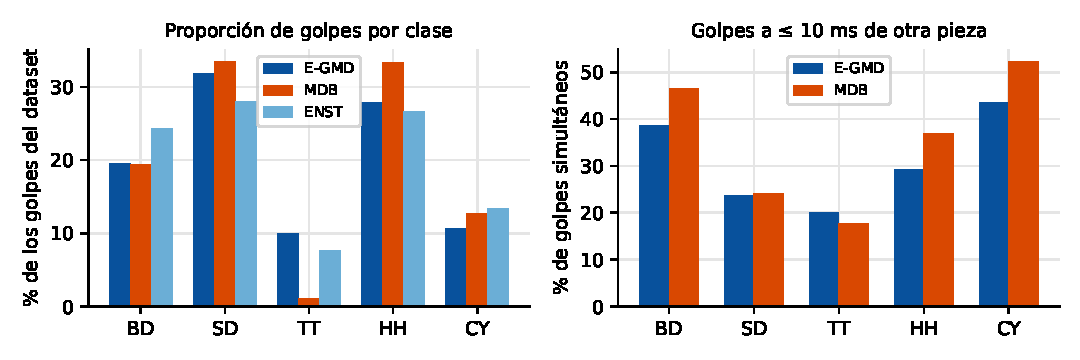
\includegraphics[width=\linewidth]{datos_cuaderno.pdf}
\caption{Izquierda: proporción de golpes por clase en cada dataset. Derecha: porcentaje de golpes que
suenan a 10~ms o menos de otra pieza.}
\label{fig:datos}
\end{figure}

\paragraph{Partición.} La partición se fijó antes de evaluar, para que los niveles 1 y 2 usen las mismas
pistas de prueba, con tres reglas: estratificada por dataset; por grupo y no por pista (canción en MDB,
baterista en ENST, para que el mismo kit no quede en ambos lados), y con la partición oficial de E-GMD.
Con semilla 0 quedaron en prueba 7 canciones de MDB (7{,}9~min), un baterista de ENST (6{,}5~min) y 123
grabaciones de E-GMD (71~min).

\paragraph{Un detalle que cambia todo.} Al comparar el modelo con el parámetro \texttt{eps} de la
normalización por lotes en $10^{-5}$ (valor por defecto de PyTorch) contra $10^{-3}$ (el de Keras, con
el que se entrenaron los pesos), la activación cambia hasta 0{,}84 y solo entre el 13 y el 63~\% de los
golpes coinciden. Ese detalle, invisible al cargar los pesos, cambia por completo la salida; el
cuaderno usa $10^{-3}$.

\subsection{Resultados del cuaderno}
La tabla~\ref{tab:nb} muestra la evaluación del nivel~1 en la partición de prueba, tal como quedó
guardada en el cuaderno. En E-GMD y MDB el modelo alcanza un $F_1$ micro de 0{,}722 y 0{,}742. En MDB
detecta casi todos los bombos (0{,}964) y bien el hi-hat (0{,}851), pero casi no los toms (0{,}050). El
0{,}722 en E-GMD es más alto que el 44{,}95 publicado; la diferencia probable es el protocolo (aquí un kit
por secuencia, cinco clases y pista solo de batería).

\begin{table}[ht]
\centering
\caption{Nivel~1 (ADTOF) en la partición de prueba del cuaderno: $F_1$ de \emph{onset} por clase y por
dataset, tolerancia de 50~ms.}
\label{tab:nb}
\begin{tabular}{lccccccc}
\toprule
\textbf{Dataset} & \textbf{BD} & \textbf{SD} & \textbf{TT} & \textbf{HH} & \textbf{CY} & \textbf{$P$ / $R$} & \textbf{$F_1$ micro} \\
\midrule
E-GMD (123 grabaciones) & 0{,}773 & 0{,}648 & 0{,}707 & 0{,}714 & 0{,}860 & 0{,}823 / 0{,}643 & 0{,}722 \\
MDB (7 canciones) & 0{,}964 & 0{,}658 & 0{,}050 & 0{,}851 & 0{,}682 & 0{,}726 / 0{,}758 & 0{,}742 \\
ENST & \multicolumn{7}{c}{\emph{no válido en esa ejecución (ver texto)}} \\
\bottomrule
\end{tabular}
\end{table}

Hay dos advertencias. La primera: la salida guardada de ENST es inválida. En esa ejecución las 76 pistas
de ENST recibieron el mismo identificador ---el código reutilizaba una variable de un bucle anterior---,
así que sus anotaciones se mezclaron y el modelo se comparó contra los golpes de todas las pistas a la
vez ($R=0{,}007$). El error se corrigió en la versión~2 del cuaderno, pero las salidas no se
regeneraron, y por la misma razón el $F_1$ global guardado (0{,}188) tampoco es válido. La segunda: las
celdas del nivel~2 están implementadas pero no se ejecutaron, así que el nivel~2 queda como diseño.

\subsection{Experimento comparativo: nivel~1 frente a MuScriptor}
\label{sec:experimento}
El cuaderno evalúa el nivel~1, pero no dice si el sistema hizo bien en reemplazarlo. Para responderlo se
comparó con el transcriptor en producción bajo un protocolo común. Se usó MDB-Drums porque es música
real producida ---el caso de uso--- y porque trae, para cada canción, la pista de solo batería y la
mezcla completa. Ninguno de los dos modelos se ajustó con estos datos, así que se evalúan las 23
canciones, además de las 7 de prueba del cuaderno por separado.

\begin{itemize}[leftmargin=1.5em]
\item \textbf{Nivel~1 (ADTOF):} el código del cuaderno sin cambios ---modelo, espectrograma, umbrales y
detección de picos--- con los pesos públicos.
\item \textbf{MuScriptor large:} el mismo binario y modelo del sistema, con el audio convertido por la
misma función del \emph{pipeline}. Sobre la mezcla se hace la pasada real del sistema (batería y bajos)
y se conservan los golpes; sobre la pista de batería se pide solo batería. Sus notas General MIDI se
llevan a las cinco clases con el mismo mapa que E-GMD.
\item \textbf{Condiciones de entrada:} (a) pista de solo batería, la condición del cuaderno; (b) pista
de batería separada por BS-RoFormer SW a partir de la mezcla, que es lo que el diseño original le daría
al nivel~1; y (c) mezcla completa, que es lo que recibe MuScriptor en el sistema.
\item \textbf{Métrica:} $F_1$ de \emph{onset} a 50~ms con emparejamiento uno a uno, micro, macro y por clase,
y tiempo de inferencia.
\end{itemize}
Por tiempo de cómputo, MuScriptor sobre la pista de solo batería se completó en 17 de las 23 canciones;
esa condición se compara aparte, sobre esas mismas 17. Los \emph{scripts} están en
\texttt{docs/report/experimento/} y los resultados por canción en \texttt{docs/report/data/}.

% ======================================================================
\section{Resultados}
\label{sec:resultados}

Los resultados se presentan del más general al más detallado: primero la comparación global en las 23
canciones, después la reproducción de las cifras del cuaderno en sus 7 canciones de prueba, luego el
análisis por canción y por tipo de error, y al final el costo de cómputo.

\subsection{Comparación global}
La tabla~\ref{tab:comp} y la figura~\ref{fig:comp} comparan las condiciones sobre las 23 canciones
(7\,924 golpes anotados). La mejor combinación es la del diseño original: \textbf{ADTOF sobre la pista
separada por BS-RoFormer SW}, con $F_1$ de 0{,}851 y $F_1$ macro de 0{,}767. Supera incluso a ADTOF sobre
la pista limpia de solo batería (0{,}844), sobre todo en precisión (0{,}849 contra 0{,}820): el separador
quita parte del sonido que el modelo confundía con golpes. Sobre la mezcla completa ADTOF baja a 0{,}796,
y MuScriptor, en la condición real del sistema, queda en \textbf{0{,}739}, con la sensibilidad más baja
(0{,}711): deja de detectar casi uno de cada tres golpes.

\begin{table}[ht]
\centering
\caption{$F_1$ de \emph{onset} en las 23 canciones de MDB-Drums. En negritas, el mejor valor de cada
columna.}
\label{tab:comp}
\small
{\setlength{\tabcolsep}{3.5pt}\begin{tabular}{llcccc|ccccc}
\toprule
& & \multicolumn{4}{c|}{\textbf{Global}} & \multicolumn{5}{c}{\textbf{$F_1$ por clase}} \\
\textbf{Modelo} & \textbf{Entrada} & $P$ & $R$ & $F_1$ & \textbf{macro} & BD & SD & TT & HH & CY \\
\midrule
ADTOF & solo batería & 0{,}820 & \textbf{0{,}869} & 0{,}844 & 0{,}744 & \textbf{0{,}965} & \textbf{0{,}819} & 0{,}216 & \textbf{0{,}862} & \textbf{0{,}859} \\
ADTOF & separada (SW) & \textbf{0{,}849} & 0{,}853 & \textbf{0{,}851} & \textbf{0{,}767} & 0{,}936 & 0{,}814 & 0{,}375 & 0{,}859 & 0{,}851 \\
ADTOF & mezcla & 0{,}777 & 0{,}817 & 0{,}796 & 0{,}719 & 0{,}818 & 0{,}742 & 0{,}357 & 0{,}844 & 0{,}834 \\
MuScriptor & mezcla & 0{,}768 & 0{,}711 & 0{,}739 & 0{,}683 & 0{,}871 & 0{,}729 & \textbf{0{,}488} & 0{,}732 & 0{,}594 \\
\bottomrule
\end{tabular}
}
\end{table}

\begin{figure}[ht]
\centering
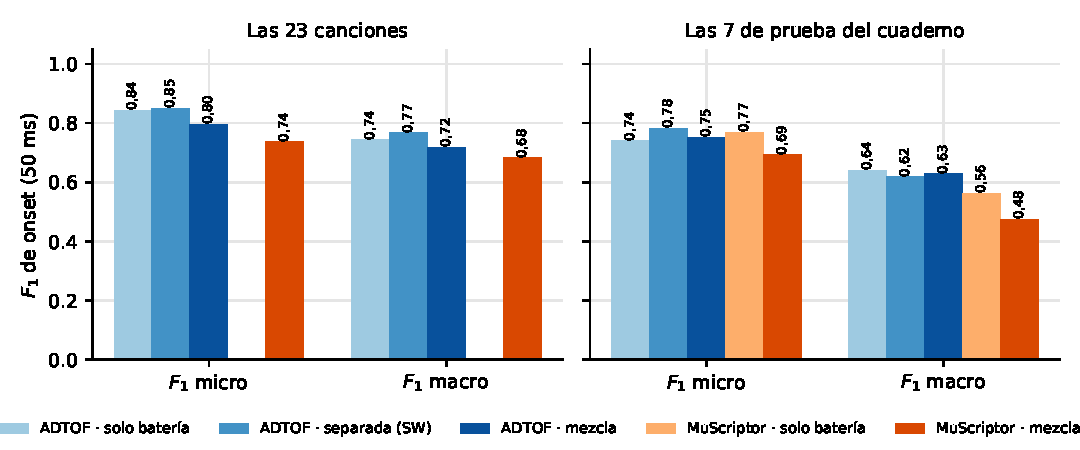
\includegraphics[width=\linewidth]{comparativa_f1.pdf}
\caption{$F_1$ micro y macro por modelo y entrada. Izquierda: las 23 canciones (MuScriptor sobre la pista
de solo batería se compara aparte, en la tabla~\ref{tab:drum17}). Derecha: las 7 canciones de prueba del
cuaderno, con las cinco condiciones.}
\label{fig:comp}
\end{figure}

Por clase (figura~\ref{fig:clases}), ADTOF es mejor en bombo, caja, hi-hat y platillos sobre la pista
separada. MuScriptor solo gana en toms (0{,}488 contra 0{,}375), una clase con apenas 90 golpes en todo
MDB. La diferencia más grande está en platillos: 0{,}851 contra 0{,}594.

\begin{figure}[ht]
\centering
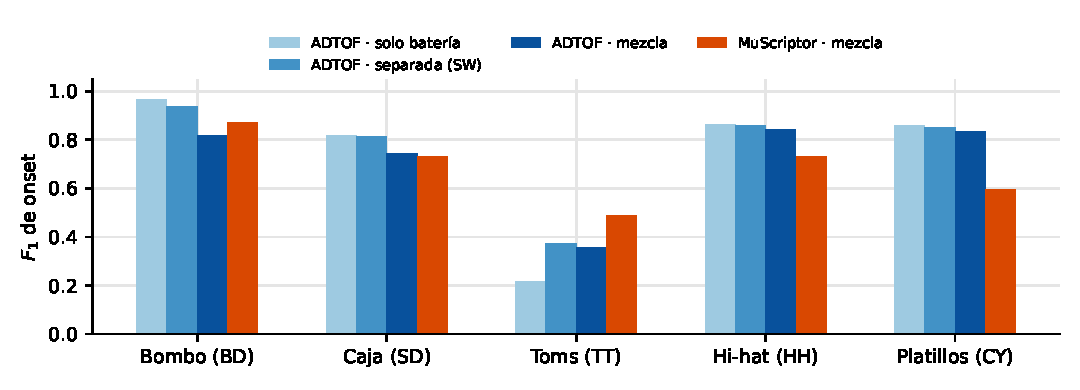
\includegraphics[width=\linewidth]{comparativa_clases.pdf}
\caption{$F_1$ por clase en las 23 canciones.}
\label{fig:clases}
\end{figure}

Con la misma pista de solo batería para ambos (tabla~\ref{tab:drum17}), las dos redes quedan cerca:
ADTOF obtiene 0{,}840 y MuScriptor 0{,}819 en $F_1$ micro, y MuScriptor gana en $F_1$ macro (0{,}785 contra
0{,}734) gracias a los toms. Es decir, MuScriptor sabe transcribir batería; lo que pierde es la capacidad
de hacerlo dentro de la mezcla, donde el bajo, las guitarras y la voz compiten con ella.

\begin{table}[ht]
\centering
\caption{Pista de solo batería, en las 17 canciones con ambos modelos.}
\label{tab:drum17}
\small
{\setlength{\tabcolsep}{3.5pt}\begin{tabular}{llcccc|ccccc}
\toprule
& & \multicolumn{4}{c|}{\textbf{Global}} & \multicolumn{5}{c}{\textbf{$F_1$ por clase}} \\
\textbf{Modelo} & \textbf{Entrada} & $P$ & $R$ & $F_1$ & \textbf{macro} & BD & SD & TT & HH & CY \\
\midrule
ADTOF & solo batería & \textbf{0{,}812} & \textbf{0{,}871} & \textbf{0{,}840} & 0{,}734 & \textbf{0{,}969} & 0{,}807 & 0{,}201 & \textbf{0{,}889} & \textbf{0{,}803} \\
MuScriptor & solo batería & 0{,}805 & 0{,}832 & 0{,}819 & \textbf{0{,}785} & 0{,}965 & \textbf{0{,}814} & \textbf{0{,}687} & 0{,}777 & 0{,}681 \\
\bottomrule
\end{tabular}
}
\end{table}

\subsection{Reproducción del cuaderno}
En las 7 canciones de prueba del cuaderno, la evaluación reproduce exactamente la cifra guardada: 2\,018
golpes acertados, 760 sobrantes y 646 faltantes, $F_1=0{,}742$, con el mismo valor en cada clase
(tabla~\ref{tab:prueba7}). Eso valida que el experimento usa el mismo modelo, pre-proceso y métrica que el
cuaderno. En este subconjunto, con mucho jazz, el orden se mantiene: ADTOF sobre la pista separada es el
mejor (0{,}783) y MuScriptor sobre la mezcla el peor (0{,}694).

\begin{table}[ht]
\centering
\caption{Las 7 canciones de prueba del cuaderno, en las cinco condiciones. La primera fila coincide
exactamente con la tabla~\ref{tab:nb}.}
\label{tab:prueba7}
\small
{\setlength{\tabcolsep}{3.5pt}\begin{tabular}{llcccc|ccccc}
\toprule
& & \multicolumn{4}{c|}{\textbf{Global}} & \multicolumn{5}{c}{\textbf{$F_1$ por clase}} \\
\textbf{Modelo} & \textbf{Entrada} & $P$ & $R$ & $F_1$ & \textbf{macro} & BD & SD & TT & HH & CY \\
\midrule
ADTOF & solo batería & 0{,}726 & 0{,}758 & 0{,}742 & \textbf{0{,}641} & 0{,}964 & 0{,}658 & 0{,}050 & 0{,}851 & \textbf{0{,}682} \\
ADTOF & separada (SW) & \textbf{0{,}828} & 0{,}743 & \textbf{0{,}783} & 0{,}620 & 0{,}934 & 0{,}651 & 0{,}040 & 0{,}871 & 0{,}605 \\
ADTOF & mezcla & 0{,}771 & 0{,}735 & 0{,}752 & 0{,}629 & 0{,}807 & 0{,}626 & \textbf{0{,}279} & \textbf{0{,}876} & 0{,}556 \\
MuScriptor & solo batería & 0{,}778 & \textbf{0{,}762} & 0{,}770 & 0{,}563 & \textbf{0{,}970} & \textbf{0{,}720} & 0{,}000 & 0{,}739 & 0{,}387 \\
MuScriptor & mezcla & 0{,}744 & 0{,}650 & 0{,}694 & 0{,}475 & 0{,}876 & 0{,}631 & 0{,}000 & 0{,}715 & 0{,}153 \\
\bottomrule
\end{tabular}
}
\end{table}

\subsection{Resultados por canción y tipo de error}
La figura~\ref{fig:cancion} compara las dos redes canción por canción. Sobre la mezcla, MuScriptor es
mejor en 9 de las 23; los mayores desacuerdos son canciones de jazz y \emph{rockabilly}. Sobre la pista de
solo batería, MuScriptor gana en 5 de 17, con diferencias pequeñas salvo en las canciones donde ADTOF
falla mucho (BebopJazz, Beatles).

\begin{figure}[ht]
\centering
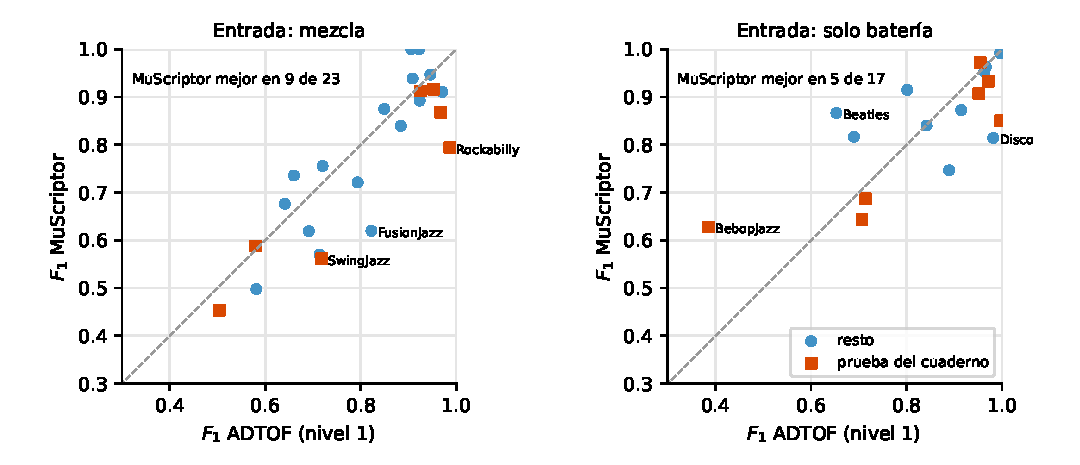
\includegraphics[width=\linewidth]{por_cancion.pdf}
\caption{$F_1$ de cada canción: ADTOF (eje horizontal) contra MuScriptor (vertical). Los puntos sobre la
diagonal son canciones donde gana MuScriptor; los cuadros naranjas son las 7 de prueba del cuaderno.}
\label{fig:cancion}
\end{figure}

La tabla~\ref{tab:confusion} explica de dónde vienen los fallos sobre la mezcla: para cada golpe anotado
que el modelo no detectó, qué clase predijo a 50~ms o menos. Dos patrones destacan. El primero es común
a ambos modelos: la mayoría de las cajas no detectadas no tienen ninguna predicción cerca. Es probable
que buena parte sean \emph{notas fantasma} ---golpes de caja muy suaves entre los golpes fuertes---, que
MDB anota como subclase propia y que suman 790 de sus 2\,654 golpes de caja. El segundo es propio de MuScriptor: confunde hi-hat y platillos en
ambos sentidos (165 hi-hats predichos como platillo y 108 platillos como hi-hat). En canciones con
\emph{ride} ---un platillo que se toca con un patrón continuo, como un hi-hat--- el modelo elige mal la
pieza aunque detecte bien el ritmo.

\begin{table}[ht]
\centering
\caption{Golpes no detectados sobre la mezcla (23 canciones) y qué predijo el modelo a 50~ms o menos de
cada uno. ``Nada'' significa que el modelo no predijo ningún golpe cerca.}
\label{tab:confusion}
\small
\begin{tabular}{llr|ccccccc}
\toprule
& \textbf{Clase anotada} & \textbf{Fallos} & \multicolumn{7}{c}{\textbf{Lo que predijo el modelo a $\le$ 50 ms}} \\
\textbf{Modelo} & & & BD & SD & TT & HH & CY & varias & nada \\
\midrule
ADTOF & Bombo & 97 & -- & 18 & 2 & 3 & 2 & 2 & 70 \\
 & Caja & 848 & 50 & -- & 36 & 37 & 7 & 44 & 674 \\
 & Toms & 28 & 2 & 5 & -- & 0 & 0 & 1 & 20 \\
 & Hi-hat & 398 & 67 & 53 & 11 & -- & 67 & 60 & 140 \\
 & Platillos & 81 & 5 & 3 & 4 & 5 & -- & 1 & 63 \\
\midrule
MuScriptor & Bombo & 187 & -- & 36 & 0 & 11 & 9 & 8 & 123 \\
 & Caja & 958 & 31 & -- & 0 & 121 & 41 & 32 & 733 \\
 & Toms & 60 & 2 & 13 & -- & 1 & 3 & 4 & 37 \\
 & Hi-hat & 696 & 24 & 109 & 0 & -- & 165 & 15 & 383 \\
 & Platillos & 387 & 11 & 42 & 0 & 108 & -- & 6 & 220 \\
\bottomrule
\end{tabular}

\end{table}

\subsection{Costo de cómputo}
La diferencia de costo es enorme. ADTOF tiene 449\,741 parámetros; MuScriptor large, unos 1{,}4 mil
millones, más de 3\,000 veces más. Sobre las 23 mezclas (21{,}8~min de audio), ADTOF tardó 228~s en la CPU
de una Apple~M2, 0{,}17 veces la duración del audio; MuScriptor tardó 6\,273~s en la GPU de la misma
máquina, 4{,}8 veces la duración del audio y unas 28 veces más que ADTOF (parte de ese tiempo compartió la
GPU con la separación). En el sistema la separación se hace de todas formas, así que usar ADTOF sobre la
pista separada no añade ese costo.

% ======================================================================
\section{Discusión}

Esta sección interpreta los resultados para la pregunta que motivó el experimento: si el sistema debe
transcribir la batería con MuScriptor o con el modelo del diseño original.

\subsection{Por qué el sistema usa MuScriptor}
La decisión de usar MuScriptor no se tomó por la batería. Un solo modelo, sin entrenamiento propio,
transcribe guitarra, bajo, piano y batería, con inicio, fin y altura de cada nota, y se puede condicionar
por instrumento. El diseño original necesitaba un modelo especializado por instrumento, cada uno con su
entrenamiento y su evaluación; con MuScriptor el sistema funcionó de punta a punta mucho antes, y el
esfuerzo se concentró en el post-proceso y la interfaz. La batería salió ``gratis'' en la misma pasada
que el bajo.

\subsection{Lo que dicen los datos sobre la batería}
Para la batería, los datos favorecen al diseño original. Sobre la pista separada, la CRNN de ADTOF supera
a MuScriptor sobre la mezcla por 0{,}112 de $F_1$ (0{,}851 contra 0{,}739), detecta más golpes
(sensibilidad de 0{,}853 contra 0{,}711) y cuesta unas 28 veces menos. La ventaja no es de capacidad: con la
misma pista limpia, ambos modelos quedan cerca. La ventaja es de \emph{entrada}: un modelo especializado
que recibe solo la batería separada trabaja en mejores condiciones que un modelo general que tiene que
encontrarla dentro de la mezcla. El separador, además, le quita a ADTOF falsas alarmas: su precisión sube
de 0{,}777 en la mezcla a 0{,}849 en la pista separada.

La recomendación es volver al diseño original solo para la batería: transcribirla con ADTOF sobre la
pista de BS-RoFormer SW y conservar MuScriptor para guitarra, piano y bajo. La tercera pasada de
MuScriptor se seguiría necesitando para el bajo, pero sus golpes de batería se descartarían. MuScriptor
solo sería mejor en toms, una clase con muy pocos ejemplos en la evaluación.

\subsection{Validez del experimento}
Hay cuatro límites. MDB-Drums tiene 23 canciones y solo 90 golpes de tom, así que las cifras de toms son
poco fiables. No se sabe si MedleyDB, de donde vienen esas canciones, está en los datos de entrenamiento
de MuScriptor; si lo estuviera, su resultado estaría inflado, lo que refuerza la conclusión. Las cinco
clases juntan \emph{crash} y \emph{ride}, y hi-hat abierto y cerrado: MuScriptor distingue más piezas, pero
esa ventaja no se mide aquí. Por último, ninguno de los dos predice intensidad: es el hueco que el nivel~2
debía cubrir.

% ======================================================================
\section{Conclusiones}

song2game muestra que es posible ir de un enlace de YouTube a una práctica interactiva de guitarra, piano
y batería con modelos abiertos y reglas explícitas. BS-RoFormer SW separa la canción en seis pistas,
MuScriptor la transcribe en tres pasadas condicionadas por instrumento, y un post-proceso con Viterbi y
límites físicos convierte las notas en tablatura y en partes de piano por mano.

El modelo de batería de nivel~1, la CRNN de ADTOF trabajada en el cuaderno del proyecto, resultó más
importante de lo que su tamaño sugiere. La evaluación reprodujo exactamente las cifras del cuaderno y,
comparada con el modelo en producción, mostró que la combinación del diseño original ---separar primero y
transcribir la batería con un modelo especializado--- obtiene el mejor $F_1$ (0{,}851), por encima de
MuScriptor sobre la mezcla (0{,}739), con una fracción del costo. Las dos lecciones son que la entrada
importa tanto como el modelo, y que un modelo general de 1{,}4 mil millones de parámetros no reemplaza
automáticamente a uno especializado de medio millón.

Por eso la arquitectura recomendada es mixta: MuScriptor para los instrumentos con altura, donde no hay
alternativa propia entrenada, y ADTOF sobre la pista separada para la batería. Con esa base, el siguiente
paso natural es ejecutar el nivel~2, para añadir la intensidad de cada golpe que hoy ningún modelo del
sistema predice.

% ======================================================================
\section{Trabajo a futuro}

Los resultados muestran que el flujo funciona de punta a punta, pero hay límites claros. La
tabla~\ref{tab:limites} los resume con su efecto y la mejora propuesta.

\begin{table}[ht]
\centering
\caption{Limitaciones conocidas y mejoras propuestas.}
\label{tab:limites}
\small
\begin{tabularx}{\linewidth}{>{\raggedright\arraybackslash}p{3.6cm}LL}
\toprule
\textbf{Limitación} & \textbf{Efecto} & \textbf{Mejora} \\
\midrule
Batería transcrita sobre la mezcla & $F_1$ de 0{,}739 contra 0{,}851 posible & Usar ADTOF sobre la pista separada (sección~\ref{sec:bateria}) \\
Sin intensidad en batería & Todos los golpes con intensidad fija (100) & Ejecutar el nivel~2, o estimarla con la pista de batería como en guitarra y piano \\
Costo de MuScriptor large & Más de una hora por canción en Docker sin GPU & Usar las versiones \emph{medium} o \emph{small} sin GPU, o el binario nativo con Metal \\
Nivel~2 sin ejecutar; ENST sin resultado válido & No se sabe cuánto aporta el ajuste fino & Regenerar las salidas de la versión~2 y entrenar el nivel~2 \\
Evaluación de batería solo en MDB & 23 canciones, 90 golpes de tom & Añadir ENST con acompañamiento e IDMT-SMT-Drums \\
Guitarra y piano sin evaluación cuantitativa & La calidad de la tablatura se juzga a oído & Medir con GuitarSet y MAESTRO mezclados y separados \\
Pesos con licencia no comercial & BS-RoFormer SW y MuScriptor son CC~BY-NC & Uso académico; para uso comercial, reentrenar o licenciar \\
\bottomrule
\end{tabularx}
\end{table}

% ======================================================================
\section{Declaración de uso de IA}

En la elaboración del proyecto se usaron herramientas de inteligencia artificial generativa como apoyo.
Gemini (Google) se usó para la revisión inicial del estado del arte en separación y transcripción. Claude
(Anthropic) se usó como apoyo en partes del código, en la preparación de los \emph{scripts} del
experimento comparativo de la sección~\ref{sec:experimento} y en la redacción y el formato \LaTeX{} de este
reporte. Las fuentes se verificaron antes de citarse, y las cifras provienen de las salidas del cuaderno y
de los resultados guardados en el repositorio.

% ======================================================================
\begin{thebibliography}{99}\small\sloppy
\bibitem{callender2020egmd} L. Callender, C. Hawthorne y J. Engel. \emph{Improving Perceptual Quality of Drum Transcription with the Expanded Groove MIDI Dataset}. arXiv:2004.00188, 2020.
\bibitem{gardner2022mt3} J. Gardner, I. Simon, E. Manilow, C. Hawthorne y J. Engel. \emph{MT3: Multi-Task Multitrack Music Transcription}. ICLR, 2022.
\bibitem{gillet2006enst} O. Gillet y G. Richard. \emph{ENST-Drums: an extensive audio-visual database for drum signals processing}. ISMIR, 2006.
\bibitem{gupta2026tart} A. Gupta et al. \emph{TART: A Modular Tool for Technique-Aware Audio-to-Tablature Guitar Transcription}. ISMIR / arXiv, 2026.
\bibitem{hawthorne2018onsets} C. Hawthorne et al. \emph{Onsets and Frames: Dual-Objective Piano Transcription}. ISMIR, 2018.
\bibitem{hawthorne2021seq2seq} C. Hawthorne, I. Simon, R. Swavely, E. Manilow y J. Engel. \emph{Sequence-to-Sequence Piano Transcription with Transformers}. ISMIR, 2021.
\bibitem{lu2023bsroformer} W.-T. Lu, J.-C. Wang, Q. Kong y Y.-N. Hung. \emph{Music Source Separation with Band-Split RoPE Transformer}. ICASSP, 2024 (arXiv:2309.02612).
\bibitem{matos2025autotab} A. Matos, D. T. B. Torres, A. Takahashi y R. B. Paradeda. \emph{AutoTab: An Interactive System for Automatic Guitar Tablature Transcription}, 2025.
\bibitem{raffel2014mireval} C. Raffel et al. \emph{mir\_eval: A Transparent Implementation of Common MIR Metrics}. ISMIR, 2014.
\bibitem{riley_adtofpytorch} X. Riley. \emph{ADTOF-pytorch}: port a PyTorch del modelo Frame RNN de ADTOF. \url{https://github.com/xavriley/ADTOF-pytorch}.
\bibitem{rouard2026muscriptor} S. Rouard, M. Krause, A. Roebel, C.-J. Simon-Gabriel y A. Défossez. \emph{MuScriptor: An Open Model for Multi-Instrument Music Transcription}. arXiv:2607.08168, 2026.
\bibitem{southall2017mdb} C. Southall, C.-W. Wu, A. Lerch y J. Hockman. \emph{MDB Drums: An Annotated Subset of MedleyDB for Automatic Drum Transcription}. ISMIR LBD, 2017.
\bibitem{toyama2023hft} K. Toyama et al. \emph{Automatic Piano Transcription with Hierarchical Frequency-Time Transformer}. ISMIR, 2023.
\bibitem{vogl2017} R. Vogl, M. Dorfer, G. Widmer y P. Knees. \emph{Drum Transcription via Joint Beat and Drum Modeling using Convolutional Recurrent Neural Networks}. ISMIR, 2017.
\bibitem{wang2023melroformer} J.-C. Wang, W.-T. Lu y M. Won. \emph{Mel-Band RoFormer for Music Source Separation}. ISMIR LBD, 2023 (arXiv:2310.01809).
\bibitem{yeung2025n2n} Yeung et al. \emph{Noise-to-Notes: Diffusion-based Generation and Refinement for Automatic Drum Transcription}. arXiv:2509.21739, 2025.
\bibitem{zehren2023adtof} M. Zehren, M. Alunno y P. Bientinesi. \emph{High-Quality and Reproducible Automatic Drum Transcription from Crowdsourced Data}. Signals, 4:768--787, 2023.
\end{thebibliography}

\end{document}
